\todo[inline]{Rewrite! New model!}

As expressed in \cref{ssec:plos}, for ~\cite{olguinmunoz:impact2021} we collected timing and task performance data for \num{40} participants performing a \num{169}-step task, guided by a \gls{WCA}, as well as personality trait scores for each participant.
For this paper, we use this data to construct a probabilistic model for the generation of realistic execution times.
The data is pre-processed to group execution time values by level of neuroticism, previous \acp{TTF}, and duration of impairment.
The resulting collections of execution times represent the distributions of these values for users with specific levels of neuroticism, interacting with systems at specific states of impairment and recent histories of impairment.
These distributions can then be sampled to produce new, realistic execution times.
In the following, we detail the step-by-step processing of this data and construction of the probabilistic model.

We employ a cleaned and re-parameterized copy of the aforementioned timing data.
The \num{6760} data points are arranged in a table together with identifiers for the subjects, their neuroticism score, and a sequence number for each step.

\begin{table}[]
    \centering
    \caption{%
        Default bins used for model parameter levels.
        For impairment, values were rounded to three decimal places.
    }
    \label{tab:defaultbins}
    % \resizebox{\columnwidth}{!}{%
    \begin{tabular}{@{}lccc@{}}
        \toprule
        \textbf{Parameter} & \textbf{Low}     & \textbf{Medium}      & \textbf{High}         \\ \midrule
        Neuroticism        & \( [0, 0.5) \)   &                      & \( [0.5, 1.0] \)      \\
        Impairment         & \( [0, 1.482) \) & \( [1.482, 3.198) \) & \( [3.198, \infty) \) \\
        Duration           & \( [0, 5) \)     & \( [5, 10) \)        & \( [10, \infty) \)    \\ \bottomrule
    \end{tabular}%
    % }
\end{table}

We begin by discretizing normalized neuroticism into \emph{low} and \emph{high} ranges, and \gls{TTF} into three ranges by splitting the data on the 3-quantiles; we will refer to these ranges of \gls{TTF} as \emph{low}, \emph{medium}, and \emph{high impairment}.
\cref{tab:defaultbins} shows the exact values used for these ranges.

The next steps of processing are slightly more complex.
For the data of each subject (which we will refer to as a \emph{run}), we shift the execution times by one sample such that each \gls{TTF} measurement (and therefore, impairment level) is associated with the execution time for the next step.
This comes directly from our discussions in \cref{sec:background} and~\cite{olguinmunoz:impact2021}.
Users notice the impairment of the current step only when they have finished it, and thus system impairment has no effect on the execution time of the current step, but directly affects the next one.

We then assign a label to each sample indicating the class of the most recent transition in impairment level in the run.
In other words, for each recorded step, we look back until we find a step with a different level of impairment and assign a label to the current step according to whether that change was from a higher to a lower level of impairment or vice-versa.
% However, if the current step is too far from the latest transition in impairment (by default, more than \num{8} steps), it is instead marked as \emph{no transition}; this label is also used for steps at the beginning of each run which have no previous transition in impairment.
% This labeling allows us to capture the behavior described in \cref{item:remain} of \cref{ssec:plos}.

Finally, we assign a number to each sample corresponding to \emph{how long} the system has been under the current level of impairment, in number of steps.
% This count resets whenever this combination changes.
This value is subsequently discretized into three levels; \emph{short}, \emph{medium}, and \emph{long duration} (again, refer to \cref{tab:defaultbins} for the exact values used).

% The results of this processing on the samples from \cref{tab:data:exectime} can be seen in \cref{tab:data:exectime:processed}.
Three examples of the effect of this discretization and processing on the data are presented in \cref{fig:timing}.
Specifically, we showcase how
\begin{enumerate*}[itemjoin={{; }}, itemjoin*={{; and}}]
    \item higher neuroticism leads to higher mean execution times as impairment goes up (\cref{fig:timing:impneurvsetime})
    \item duration has both a speed-up and slow-down effect on execution times, depending on the level of impairment (\cref{fig:timing:durvsetime})
    \item transitions from higher to lower levels of impairment lead to higher mean execution times when compared to steps far away from a transition, or from a transition from lower to higher levels of impairment (\cref{fig:timing:imptransvsetime})
\end{enumerate*}.


Finally, we present a step-by-step breakdown of how this data is subsequently used to generate realistic execution times.
A model which uses this processed data to generate execution times needs to maintain variables for duration, previous impairment, and most recent transition.
At the beginning of each step, it:
\begin{enumerate}
    \item Checks whether any change in impairment has occurred.
          If it has, it resets duration to \num{1} and updates the transition variable accordingly.
          If not, it increases the duration variable by one.
        %   unless that increase causes it to exceed the threshold of steps required to forget a transition.
        %   If that's the case, instead the model resets duration to \num{1} and sets the transition variable to ``no transition''.
    \item Discretizes the updated duration value.
    \item Finds all samples with binned neuroticism, impairment and duration matching the state of the system.
    If, and only if, the current duration falls within the \emph{short} duration bin, this data is further bisected according to the current value of the transition variable.
    \item Randomly samples the filtered data to obtain a realistic execution time value.
          \begin{itemize}
              \item Alternatively, a distribution can be first be fitted to the filtered samples.
                    The model then samples the theoretical distribution instead of the empirical samples.
          \end{itemize}
    \item Finally, updates the stored impairment value with the new impairment and proceeds to the next step.
\end{enumerate}

We use Python~\num{3.10} to implement two variants of the above described timing model.
The first of these samples execution times directly from the empirical data from~\cite{olguinmunoz:impact2021}; we will refer to it hereafter as the \emph{empirical model}.
The second corresponds to one which first fits a theoretical \gls{exGaussian} distribution to the data before sampling; we will refer to this one as the \emph{theoretical model}.
The \gls{exGaussian} distribution was chosen due to the vast body of research supporting its suitability for the modeling of the timing of human actions~\cite{Rohrer1994analysis,Palmer2011shapes,Marmolejo2022generalised}.
Collectively, we will refer to both these models interchangeably as the \emph{realistic models} or \emph{second-order models}.
\todo[inline]{Explain why using ExGaussian?}

We also implement two simpler reference timing models:
\begin{enumerate*}[itemjoin={{; }}, itemjoin*={{; and }}]
    % \item a model which returns a constant execution time, corresponding to the mean execution time of all samples associated with the lowest impairment and the shortest duration
    \item a model which randomly samples from the raw data without any grouping
    \item a model which fits an \gls{exGaussian} distribution to the raw data, without any grouping, and then randomly samples from it
\end{enumerate*}.
We will refer to these models individually as the \emph{naive} and \emph{fitted-naive} model, respectively, and collectively as the \emph{firt-order models}.

\begin{figure*}
    \centering
    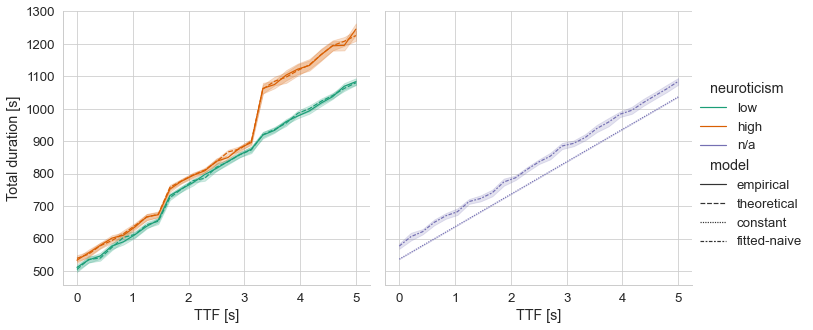
\includegraphics[width=.9\textwidth]{figs/model_comp_controlled_ttf.png}
    \begin{tabular}{ll >{\columncolor[HTML]{EAEAEA}}r >{\columncolor[HTML]{EAEAEA}}r rr}
    \toprule
    {} & {} & \multicolumn{2}{>{\columncolor[HTML]{EAEAEA}}c}{\gls{TTF} \( = \) \SI{0}{\second}} & \multicolumn{2}{c}{\gls{TTF} \( = \) \SI{5}{\second}} \\
    {Model} & {Neuroticism} & {Total Duration} & {Diff.\ w.r.t.\ fitted-naive} & {Total Duration} & {Diff.\ w.r.t.\ fitted-naive} \\
    \midrule
    fitted-naive & & \SI{575.54}{\second} & & \SI{1082.28}{\second} & \\
    \multirow[c]{2}{*}{empirical} & low & \SI{509.39}{\second} & \SI{-11.49}{\percent} & \SI{1071.99}{\second} & \SI{-0.95}{\percent} \\
    & high & \SI{536.48}{\second} & \SI{-6.79}{\percent} & \SI{1235.65}{\second} & +\SI{14.17}{\percent} \\
    \multirow[c]{2}{*}{theoretical} & low & \SI{505.22}{\second} & \SI{-12.22}{\percent} & \SI{1073.49}{\second} & \SI{-0.81}{\percent} \\
    & high & \SI{536.31}{\second} & \SI{-6.82}{\percent} & \SI{1235.70}{\second} & +\SI{14.18}{\percent} \\
    \bottomrule
    \end{tabular}
    \caption{
        Comparison of the total duration of \num{100}-step tasks for different models in the controlled \gls{TTF} setup.
        The table shows a detailed breakdown of durations for the fitted-naive, empirical, and theoretical models at the lowest and highest \acp{TTF}, as well as relative differences with respect to the corresponding fitted-naive baseline for each case.
    }\label{fig:ctrlttf}
\end{figure*}


We first compare these models using a controlled, ideal setup with \num{25} constant, linearly distributed \acp{TTF} in the \SIrange[]{0}{5}{\second} range.
For each \gls{TTF}, the models execute \num{30} independent repetitions of a \num{100} step task.

We show the results of these runs in \cref{fig:ctrlttf}.
Two interesting behaviors of the realistic models can be noticed in this plot.
One, all realistic models are faster than the reference models at the lowest \gls{TTF}.
When compared to the fitted-naive model, the reduction in total duration was on average \textasciitilde\SI{12}{\percent} for realistic models with low neuroticism, and \textasciitilde\SI{6.8}{\percent} for the same models with high neuroticism.

Two, at the highest \gls{TTF}, \emph{only} the high neuroticism models show any significant difference in duration with respect to the reference models.
For \gls{TTF} \(=\) \SI{5.0}{s}, the high neuroticism realistic models were on average \textasciitilde\SI{14.18}{\percent} slower than the fitted-naive model, whereas the low neuroticism models showed no significant relative difference in duration.

These behaviors clearly stem from the effects identified in \textcite{olguinmunoz:impact2021}, described in \cref{ssec:plos}.
At low levels of impairments, i.e.\ small \acp{TTF}, the speed-up effect dominates, bringing execution times to a minimum and consequently resulting in shorter total durations.
On the other hand, at high levels of impairment, the slow-down (pacing) effect starts to take over, pushing step execution times and total durations up.
However, only in the high neuroticism case do execution times eventually surpass the reference model, which is in line with our findings with respect to the modulating effects of neuroticism.

\medskip

\begin{figure}
    \centering
    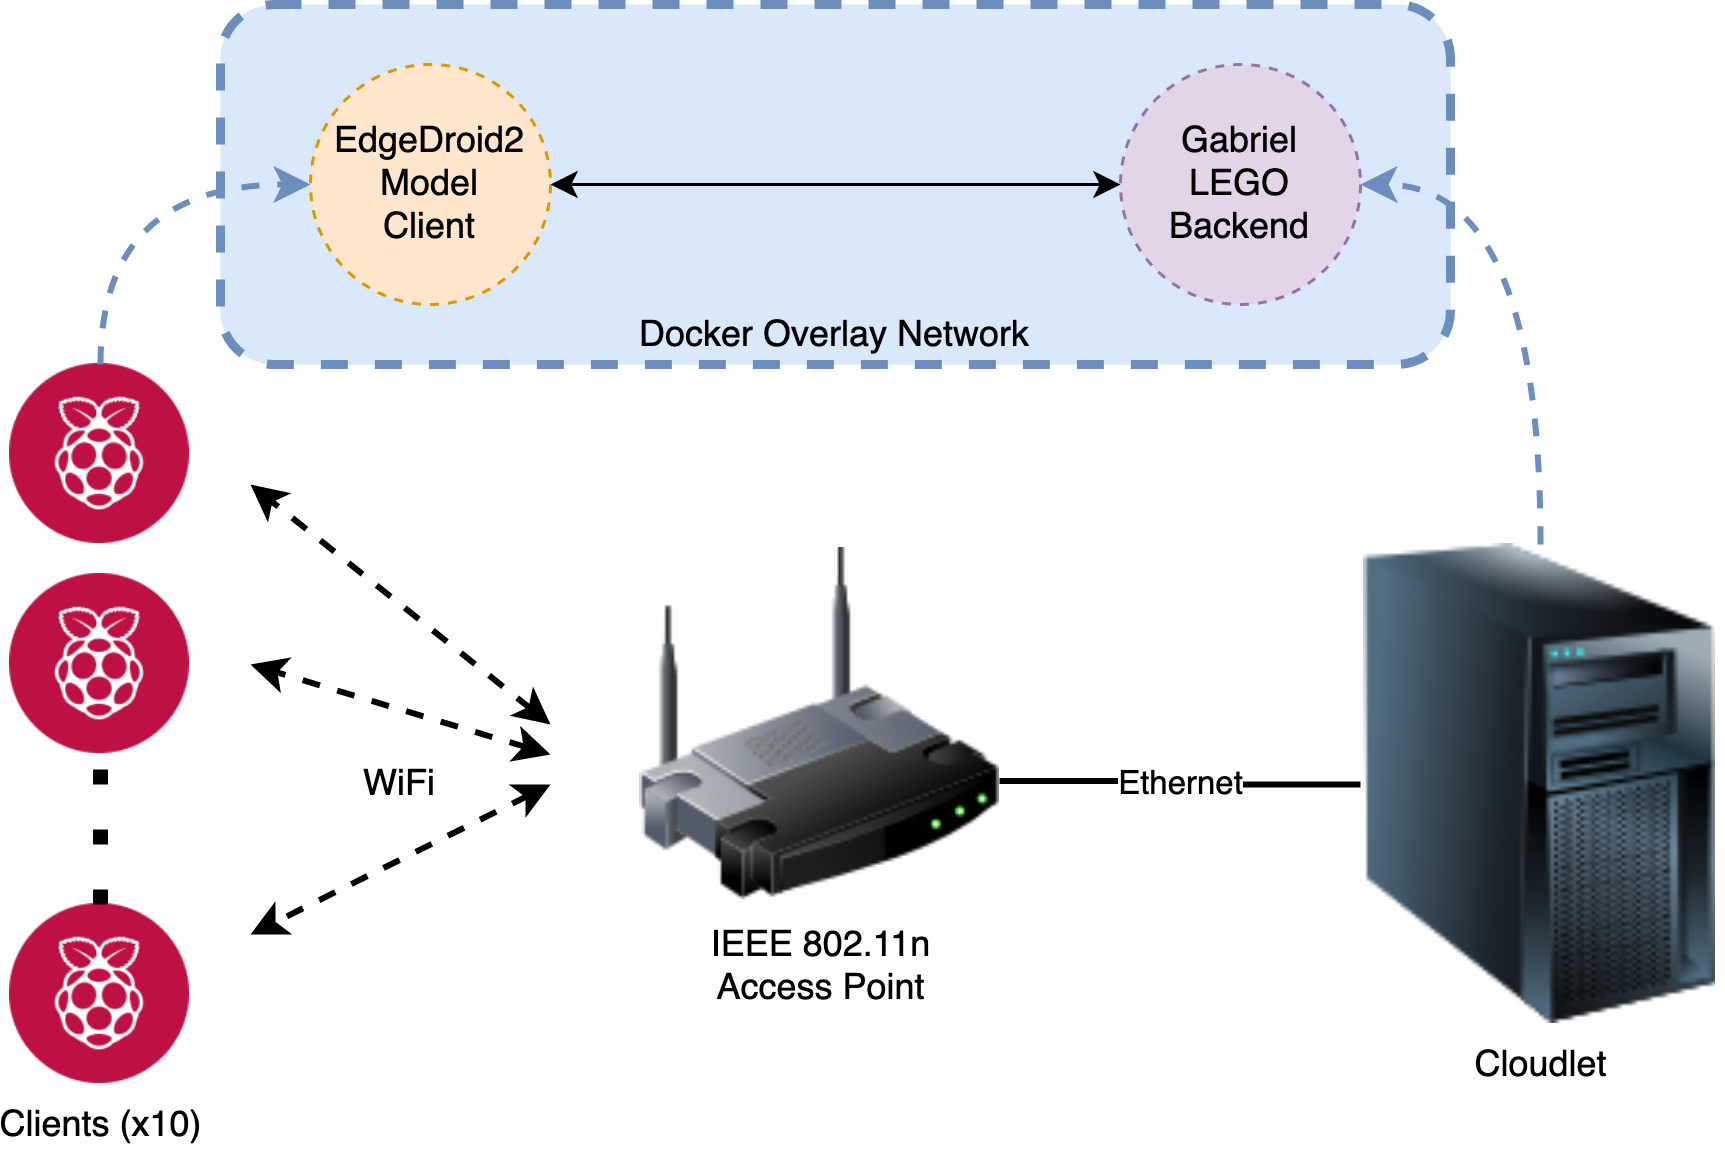
\includegraphics[width=\columnwidth]{figs/EdgeDroid2ExperimentalSetup.png}
    \caption{%
        Experimental setup used to study the implications of the realistic models of human behavior for \gls{WCA}.
        We deploy containerized instances of the client-server loop running the models on a testbed consisting of \num{10} Raspberry Pi clients connected to a cloudlet over a \gls{COTS} \acs{IEEE} \num{802.11}n access point.
    }\label{fig:expsetup}
\end{figure}

These models are then integrated into client software for communicating with an adapted and instrumented version of the Gabriel~\cite{Chen2015LEGO,Chen2018application} \gls{WCA} backend running variants of the LEGO task.
In the following we use these client-server loops together with the testbed show in \cref{fig:expsetup} to illustrate the implications of the realistic timing models.
Our goal is to understand the consequences of taking second order effects into consideration when modeling execution times, versus simply relying on first-order statistics.

\todo[inline]{Update with new deployment, 802.11b/g wifi.}

We deploy an increasing number of client-server loops (\numlist{1;4;7;10} loops) in parallel on the testbed and record the resulting timing metrics.
These setups are repeated \num{5} times per model for better statistical representativeness; realistic models parameterized with \emph{low} (\num{0.0}) and \emph{high} (\num{1.0}) neuroticism are considered separate models for the purpose of this experiment.
The task used for all repetitions corresponds to a variant of the \num{169}-step tasks used in~\cite{olguinmunoz:impact2021}, truncated to \num{45} steps plus a special initial trigger step. 

\medskip

\begin{figure*}
    \centering
    \begin{subfigure}[t]{\columnwidth}
        \centering
        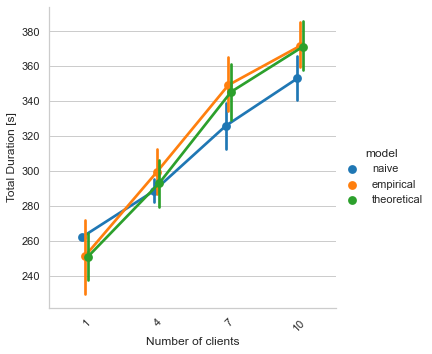
\includegraphics[width=.8\textwidth]{figs/numclients_vs_duration.png}
        \caption{%
            Consequences of decreased system responsiveness due to resource and network congestion.
            At lower levels of resource contention, the realistic models outperform the naive one due to the speed-up effect described in \cref{sec:background}.
            However, at higher levels of contention, the behavioral slow-down of the realistic models due to higher \acp{TTF} takes over.
        }\label{fig:scaling_duration}
    \end{subfigure}%
    \hspace{\fill}%
    \begin{subfigure}[t]{\columnwidth}
        \centering
        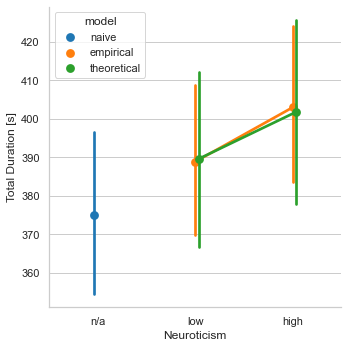
\includegraphics[width=.8\textwidth]{figs/neuroticism_vs_duration.png}
        \caption{%
            Modulating effects of neuroticism on task duration.
            Realistic models parameterized with high neuroticism are on average \SI{7.3}{\percent} slower than the reference model, and \SI{3.37}{\percent} slower than the same models instead parameterized with low neuroticism.
        }\label{fig:neuro_duration}
    \end{subfigure}%
    \caption{Results for both scenarios described in \cref{ssec:model:verification}. Error bars indicate the \SI{95}{\percent} \gls{CI}.}
\end{figure*}

\cref{fig:scaling_duration} illustrates the results for scenario \labelcref{verification:scaling}.
It showcases the important behaviors of the realistic models which are not captured by the naive, non-adaptive model.
On one hand, the realistic models (and by extension, humans) are actually faster than the naive model by up to \SI{4.37}{\percent} in a deployment with no resource contention.
This is due to the speed-up effect described in \textcite{olguinmunoz:impact2021} --- humans get faster as a task progresses with a high system responsiveness.

On the other, the realistic models experience a mean slowdown of about \SI{5.13}{\percent} at the highest level of resource contention (\num{10} concurrent loops) when compared to the naive model, even though only about \SI{22}{\percent} of \acp{TTF} in this scenario reach the medium impairment level and practically no \acp{TTF} pass threshold for the highest level of impairment.
This showcases that the additional user slow-down due to reduced system responsiveness, originally described in \textcite{olguinmunoz:impact2021}, causes a noticeable and significant extension of system utilization time, even at lower and medium levels of impairment.

\medskip

We illustrate the results of scenario \labelcref{verification:neuro} in \cref{fig:neuro_duration}, showcasing the modulating effects of neuroticism in a medium-impairment setup.
The realistic models were on average \SI{3.8}{\percent} slower than the reference naive model when configured with a low level of neuroticism, and \SI{7.3}{\percent} slower when configured with a high neuroticism.
In this scenario, an average of \SI{50}{\percent} of all recorded \acp{TTF} fell within the medium impairment range, and about \SI{26.6}{\percent} within the high impairment range, showing that the effects of behavioral slow-down are considerable even in moderately impaired systems. 

\medskip

The results for scenarios \labelcref{verification:scaling,verification:neuro} showcase the importance and potential impact of realistic models for the study of \gls{WCA} applications.

\todo[inline]{Finish this subsection.}